\documentclass[11pt]{paper}

\usepackage{preamble}

%%% section divider;
%\newcommand{\secdiv}{\begin{center}
%\adforn{21}\quad\adforn{11}\quad\adforn{49}
%\end{center}
%}



%%%% Important sets
\newcommand{\setOfReals}{\mathbb{R}}
\newcommand{\setOfNaturals}{\mathbb{N}}
\newcommand{\setOfNonnegativeIntegers}{{\mathbb{N}_0}}
\newcommand{\setOfPositiveReals}{{\setOfReals_{+}}}
\newcommand{\setN}[1]{ [ #1]}
\newcommand{\setTime}[1]{\mathcal{T}_{#1}}

\newcommand{\borel}[1]{\mathcal{B} (#1 )}
\newcommand{\setOfMeasures}[2]{\mathcal{M}_{#2}\left(#1\right)}
\newcommand{\setOfProbabilityMeasures}[1]{\mathcal{P}\left(#1\right)}
\newcommand{\setOfContinuous}[2]{{C}\left(#1, #2\right)}
\newcommand{\setOfBoundedContinuous}[2]{{C}_{b}\left(#1, #2\right)}
\newcommand{\setOfBoundedDifferentiable}[2]{{C}_{b}^{(1)}\left(#1, #2\right)}
\newcommand{\setOfcadlag}[2]{{D}\left(#1, #2\right)}
\newcommand{\setOfcompactSupported}[2]{C_{K}\left(#1, #2\right)}
\newcommand{\setOfBoundedMeasurable}[2]{{B}_{b}\left(#1, #2\right)}


\newcommand{\BigO}[1]{\mathop{}\!O{\left(#1\right)}}
\newcommand{\smallO}[1]{\mathop{}\!o{\left(#1\right)}}




% generic system names
\newcommand{\sys}[1]{\textsc{#1}}





%\newcommand{\supp}{{\mathrm{supp}}  }
%\def\bD{\boldsymbol\Delta}
%\def\L{{\cal L}}

% \def\C{{\mathbb C}}
% \def\eps{\epsilon}
%\def\S{\ensuremath{\mathrm{S}}}
%\def\I{\ensuremath{\mathrm{I}}}
%\def\R{\ensuremath{\mathrm{R}}}
% \def\var{\mathbb{V}\mathrm{ar}}
% \def\cov{\mathbb{C}\mathrm{ov}}
% \def\corr{\mathbb{C}\mathrm{orr}}
% \def\la{\lambda}
% \def\ga{\gamma}
% \def\Rn{{\cal R}_0}
% \def\io{\iota}
% \def\ro{\Rn}
% \def\tS{\tilde S}
% \def\nn{\nonumber}
% \def\th{\theta}
% \newcommand\ind[1]{\mathbb{I}_{#1}}
%
% \newcommand\be{\begin{equation}\label}
%\newcommand\ee{\end{equation}}
%
% \def\G{{\cal G}}
% \def\d{\partial}
%
% \def\c{\circ}
% % % % Probability distributions

% % % Distributions
\newcommand{\Bin}[2]{\sys{Binomial}(#1, #2 )}
\newcommand{\Poi}[1]{\sys{Poisson} (#1)}


% % % % Functions
\newcommand{\measureIntegral}[2]{#1\left(#2 \right) }
%\newcommand{\measureIntegral}[2]{\langle#1, #2 \rangle }

\newcommand{\optionalVariation}[1]{ [#1] }
\newcommand{\predictableVariation}[1]{ \langle#1\rangle }

\newcommand{\cardinality}[1]{\mid #1  \mid}

\DeclarePairedDelimiter\ceil{\lceil}{\rceil}
\DeclarePairedDelimiter\floor{\lfloor}{\rfloor}

\DeclarePairedDelimiter\abs{\lvert}{\rvert}
% Swap the definition of \abs* and \norm*, so that \abs
% and \norm resizes the size of the brackets, and the
% starred version does not.
\makeatletter
\let\oldabs\abs
\def\abs{\@ifstar{\oldabs}{\oldabs*}}
%

\newcommand{\cadlag}{c\`adl\`ag\,}

\newcommand{\aggregation}[1]{\mathsf{agg}\left( #1  \right)}
\newcommand{\uniformization}[1]{\mathsf{unif}\left( #1  \right)}
\newcommand{\fibre}[1]{\mathsf{fibre}\left( #1 \right)}

\newcommand{\SymmetryGroup}[1]{\mathsf{Sym}\left( #1 \right)}

\newcommand{\Aut}[1]{\mathsf{Aut}\left( #1 \right)}

\newcommand{\coset}[2]{\langle #1 \rangle_{#2}}

\newcommand{\KL}[2]{D_\mathrm{KL}\left( #1 \mid\mid #2  \right) }


%\newcommand{\metricGivenSpace}[3]{\rho_{#3} \left( #1, #2  \right) }
\newcommand{\metricGivenSpace}[1]{\mathsf{d}_{#1} }

\newcommand{\etal}{\textit{et al.}}

\newcommand{\wrt}{\textit{w.r.t.\ }}


\newcommand{\clip}[1]{\,\mathsf{clip} \left(#1 \right)}

\renewcommand{\vec}[1]{\mathbf{#1}}
\newcommand{\mat}[1]{\mathrm{\mathbf{#1}}}
\newcommand{\Cov}[1]{\mathsf{Cov}(#1)}
\newcommand{\Corr}[1]{\mathsf{Corr}(#1)}
\newcommand{\diag}[1]{\mathrm{diag}(#1)}

\DeclareMathOperator*{\esssup}{ess\,sup}


\newcommand{\defeq}{\coloneqq}

\newcommand{\identity}{\mathsf{Id}}

\newcommand{\indicator}[1]{\mathsf{1}_{#1}}

\newcommand{\FOperator}[2]{\mathsf{A}_{#2} (#1) }
\newcommand{\HOperator}[2]{\mathsf{C}_{#2} ( #1) }
\newcommand{\GOperator}[2]{\mathsf{B}_{#2} ( #1) }


\newcommand{\JOperator}[1]{\mathsf{J}( #1) }
\newcommand{\UOperator}[1]{\mathsf{U}( #1) }
\newcommand{\VOperator}[1]{\mathsf{V}( #1) }

\newcommand{\myOperator}[1]{\mathsf{#1}}


\newcommand{\Permanent}[1]{\mathsf{per} \hspace{2pt} #1}
\newcommand{\allpermutations}[1]{\Theta (#1)}
\newcommand{\diophantine}[2]{\Lambda (#1,#2)}

\newcommand{\projection}[2]{\mathbbm{P}_{#1}{\left( #2 \right)}}

\newcommand{\diffOperator}[2]{\mathbbm{D}^{#2}#1}
\newcommand{\differential}[1]{\,\mathrm{d} #1}
\newcommand{\timeDerivative}[1]{\frac{\differential}{\differential t} #1 }
\newcommand{\partialDerivative}[2]{\frac{\partial}{\partial #2} #1 }

\newcommand{\interior}[1]{ \mathsf{Int} \, #1 }
%\newcommand{\closure}[1]{ \mathsf{Cl} \, #1 }
\newcommand{\closure}[1]{ \overline{ #1 } }
%\newcommand{\boundary}[1]{\mathsf{Bnd}\, #1}
\newcommand{\effectiveDomain}[1]{\mathsf{dom}\, #1}

\newcommand{\range}[1]{ \mathsf{rng} \left(#1\right)  }

\newcommand{\eqstop}{.}
\newcommand{\eqcomma}{,}


\newcommand{\norm}[2]{\left\lVert#1\right\rVert_{#2}}

\newcommand{\E}{\mathsf{E}}
\newcommand{\Eof}[1]{\E\left[#1 \right]}
\newcommand{\EofP}[2]{\E_{#1}\left(#2\right)}

\newcommand{\V}{\mathsf{Var}}
\newcommand{\VarOf}[1]{\V\left[#1\right]}
\newcommand{\VarOfP}[2]{\V_{#1}\left(#2\right)}

\newcommand{\NPermuteR}[2]{ (  #1)_{#2}  }

\newcommand{\prob}{\mathsf{P}}
\newcommand{\probOf}[1]{\prob\left(#1\right)}

\newcommand{\given}{\mid}

\newcommand{\history}[1]{\mathcal{F}_{#1}  }

\newcommand{\trans}{^{\mathsf T}}

\newcommand{\disteq}{\, \overset{\mathcal{D}}= \, }

\newcommand{\ConvInProb}{\xrightarrow[]{ \hspace*{4pt}  \text{         P   } }}
\newcommand{\ConvAlmostSure}{\xrightarrow[]{ \hspace*{4pt}  \text{         a.s.   } }}
\newcommand{\ConvInDist}{  \overset{\hspace*{4pt}  \mathcal{D}  }{\implies } }


\DeclareMathOperator*{\Bigcdot}{\bullet}


\newcommand{\myExp}[1]{\exp \left( #1 \right)  }

\newcommand{\ie}{\textit{i.e.}}
\newcommand{\eg}{\textit{e.g.}}
\newcommand{\ia}{\textit{i.a.}}
\newcommand{\viz}{\textit{viz.}}
\newcommand{\vide}{\textit{vide}}

\newcommand{\quotes}[1]{``#1''}




% TODO-Package with author-macroscd
% \usepackage{todonotes}
% \usepackage{ifthen}
%  \newboolean{draftversion}
% \setboolean{draftversion}{true} %set false for removing comments and watermark
%
%
 %\newcommand{\wasiur}[2]{\ifthenelse{\boolean{draftversion}}{\todo[inline, color=tud1a!50, caption={2do}, #1]{\begin{minipage}{\textwidth-4pt}\emph{Remark Wasiur:}\\#2\end{minipage}}}{}}
%
% \newcommand{\eben}[1]{\ifthenelse{\boolean{draftversion}}{\todo[inline, color=tud1a!50, caption={2do}, #1]{\begin{minipage}{\textwidth-4pt}\emph{Remark Eben:}\\#2\end{minipage}}}{}}
%
% \newcommand{\greg}[1]{\ifthenelse{\boolean{draftversion}}{\todo[inline, color=tud1a!50, caption={2do}, #1]{\begin{minipage}{\textwidth-4pt}\emph{Remark Greg:}\\#2\end{minipage}}}{}}
%
%
%
% \ifthenelse{\boolean{draftversion}}{\usepackage[firstpage]{draftwatermark}}{}

\newcommand{\eben}[1]{\textcolor{tud7a}{$\langle${\slshape{\bfseries Eben:} #1}$\rangle$}}
\newcommand{\wasiur}[1]{\textcolor{tud9d}{$\langle${\slshape{\bfseries Wasiur:} #1}$\rangle$}}
\newcommand{\gr}[1]{\textcolor{tud3a}{$\langle${\slshape{\bfseries Greg:} #1}$\rangle$}}



%%% equation numering
\renewcommand {\theequation}{\arabic{section}.\arabic{equation}}

\pagestyle{plain}
\pagenumbering{arabic}

% \titlespacing\section{0pt}{10pt plus 4pt minus 2pt}{6pt plus 2pt minus 2pt}
% \titlespacing\subsection{0pt}{8pt plus 4pt minus 2pt}{3pt plus 2pt minus 2pt}
% \titlespacing\subsubsection{0pt}{6pt plus 4pt minus 2pt}{2pt plus 2pt minus 2pt}
% \titlespacing{\paragraph}{0pt}{5pt plus 2pt minus 2pt}{2pt plus 2pt minus 2pt}
% %\setlength\parindent{.1 cm}


\newcounter{ocounter}
\newcounter{acounter}
\setlength{\parskip}{0pt}


\title{The Impact of Age, Education, Marital Status and Sex on Wage and Salary Income}
\author{\color{tud1d}\sffamily Kai Li\thanks{Department of Mathematics, The Ohio State University, USA, email: \href{mailto:li.8130@osu.edu}{li.8130@osu.edu}}\quad
\color{tud1d}\sffamily Sicong Wang\thanks{Fisher College of Business, The Ohio State University, USA, email: \href{mailto:wang.8810@osu.edu}{wang.8810@osu.edu}}\quad
\color{tud1d}\sffamily Zeer Kang\thanks{Department of Mathematics, Economics, The Ohio State University, USA, email: \href{mailto:kang.1063@osu.edu}{kang.1063@osu.edu}}
}


\begin{document}

\maketitle

\abstract{This paper explores the relationship between multiple explanatory variables, marital status, age, sex, education and birthplace (born in the United States or not), and the explained variable income. Motivated by the classical \acp{MLR} and \acp{MNR}, we analyze the given reliable data and find out the best-fitted model of these variables using the \ac{OLS} technique by software Stata. The regression results from Stata enable us to easily understand and interpret how these regressors affect the regressand through statistical inference.}

\keywords{econometrics, data analysis, \ac{MLR}, \ac{MNR}, Stata, statistical inference}

\abovedisplayskip=6pt
\belowdisplayskip=6pt

\section{Introduction}
\label{sec:intro}

Nowadays, people may wonder about factors that can lead to higher salaries. Economists have already done lots of empirical analysis on this topic. The objective of the paper is to perform similar empirical research among multiple interested predictor variables \textit{Age}\footnote{We \textit{italicize} the variables in our model in the paper.}, \textit{Education}, \textit{Male}, \textit{Nonmarried}, \textit{US}, and a predicted variable \textit{Wage} using a data set from \acs{CPS}. We treat ordinal variables approximately continuous in our regression model. By performing such a regression analysis, we can analyze and interpret how selected factors can affect salary. More importantly, we, or economists, are able to explain social, economic issues such as gender, birthplace discrimination, income distribution, and the importance of education to future earnings. Thus, this empirical research provides meaningful insights on applications to economics and statistics.

For the rest of the paper, we first filter out irrelevant variables and observations from the data in \hyperref[sec:data]{\text{Data}} Section. Then, we shall provide a rough estimate of what the fittest model looks like in \hyperref[sec:em]{\text{Empirical Methodology}} Section.  Starting from assuming an \acs{MLR} model, we expand our regression model to \acs{MNR} and measure its goodness of fit. Then, we analyze the data and select a model that represents our data set most effectively and accurately using \acs{OLS} estimators obatined from Stata, shown in \hyperref[sec:results]{\text{Results}} Section. Also, we conclude the statistical significance of the coefficients and interpret the results. Before doing the analysis, we predict nonlinear relationships between \textit{Wage} and \textit{Age}, \textit{Education}. Finally, notations, mathematical proofs of the \acs{OLS} formula and \acs{GMT} verifications are provided in Appendix \ref{appendix:math}.

\setcounter{equation}{0}
\section{Data}
\label{sec:data}

One critical step is to inspect the reliability of the data set before using the data for analysis. The data set is a subsample of the \ac{CPS}. The \acs{CPS}, sponsored jointly by the U.S. Census Bureau and the U.S. Bureau of Labor Statistics, is the primary source of labor force statistics for the population of the United States. The \acs{CPS} is one of the oldest, largest, and most well-recognized surveys in the United States \cite{ipums_2020}. We also examined the statistical sampling techniques and designs of \acs{CPS}. Therefore, it is reasonable to believe the data set will provide reliable information.

We eliminate \textit{Year} and \textit{Month} in our data to reduce the complexity of working with panel data. Outliers are also narrowed out after drawing the Box-and-Whisker plots in Stata to preserve integrity. After that, we obtain summary statistics (see Table \ref{tab:summary_statistics}) and scatterplots of the ordinal variables in matrix form (see Figure \ref{fig:matrix}). Our data set contains a variety of people whose annual ages are mostly in range 14000 to 78000, aging from 21 to 63 with education level from 5th-grade to doctoral, given the means and the standard deviations. Whether people are male, nonmarried, or born in the US are included for our economic interests as well. 

\begin{table}
\scriptsize
\begin{adjustbox}{width=\textwidth}
\begin{tabular}{l*{1}{ccccc}}

\hline\hline

Variables\footnotemark   & Observation&        Mean&Standard Deviation&         Min&         Max\\
\hline
Wage        &       71800&    45570.07&       26987.01&        6740&  120000\\
Age         &       71800&       42.31&          13.92&          15&       85\\
Education   &       71800&       89.52&          22.17&          20&      125\\
Male        &       71800&        0.51&           0.50&           0&        1\\
Nonmarried  &       71800&        0.30&           0.45&           0&        1\\
US          &       71800&        0.81&           0.39&           0&       1\\
\hline\hline

\end{tabular}
\end{adjustbox}
\caption{\label{tab:summary_statistics}
Summary statistics for the research variables.}
\end{table}

\footnotetext{\textit{Wage} and \textit{Education} are ordinal variables. The higher the number, the higher the salary or degree.}
\footnotetext{\textit{Male}, \textit{Nonmarried} and \textit{US} are indicator variables. See the Code Book for specifics in Reference \cite{ipums_2020}.}


\begin{figure}[htp]
  \centering
  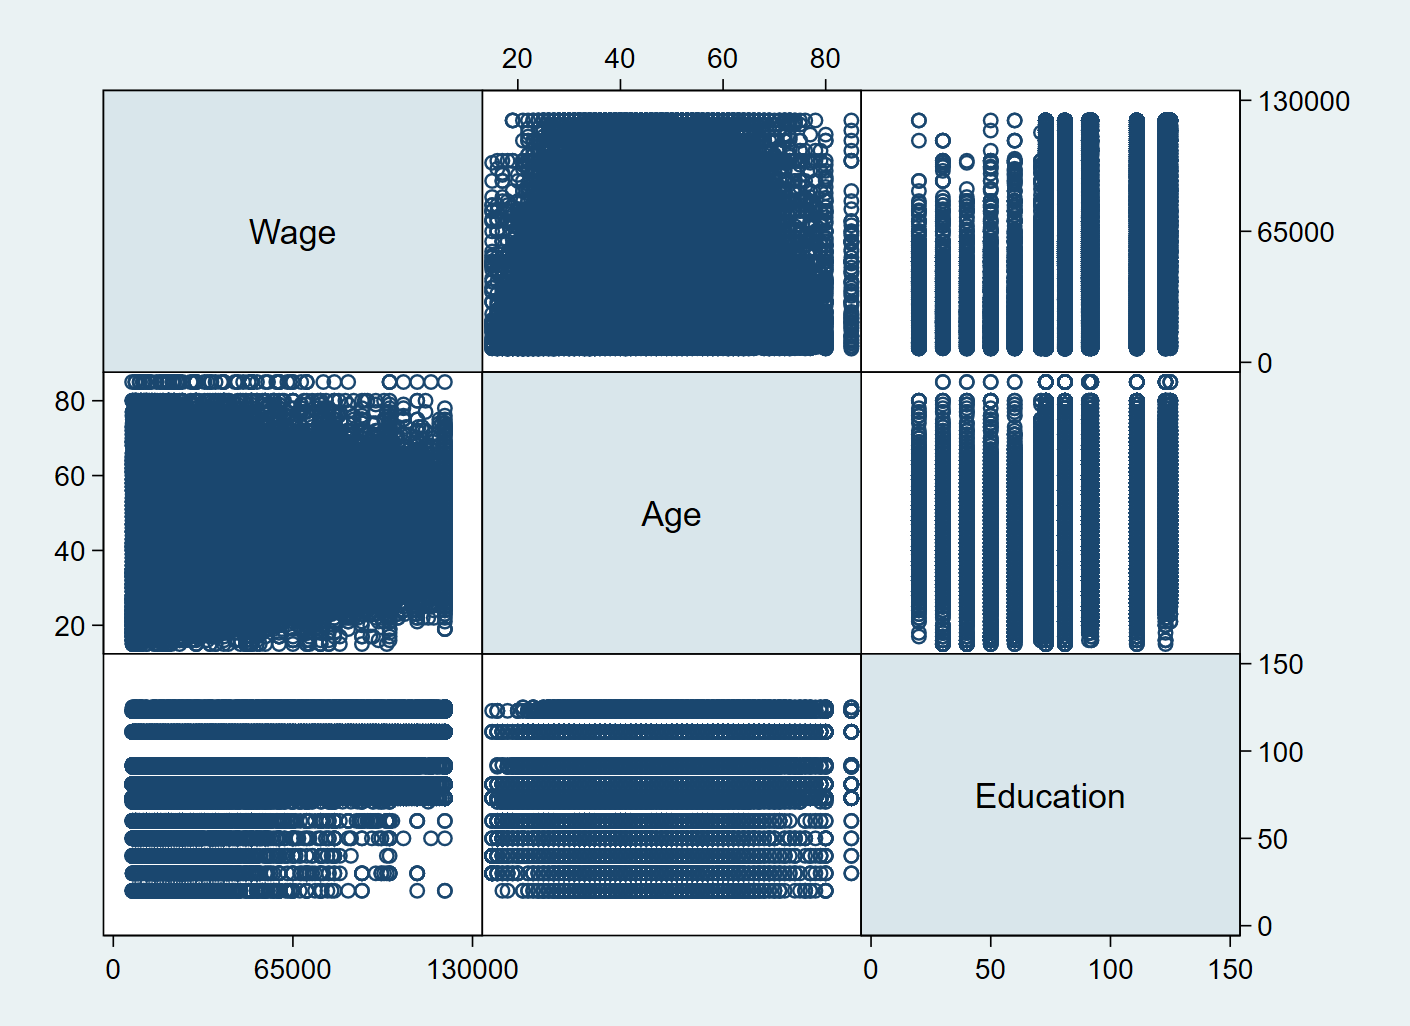
\includegraphics[scale=0.2]{{figures/graph_matrix}}
  \caption{\label{fig:matrix}
  \textit{graph matrix}\protect\footnotemark of approximately continous regression variables
   }
\end{figure}

\footnotetext{\textit{graph matrix} is a Stata command used to draw a scatterplot matrix to illustrate the bivariate relationships.}

\noindent We came up with the following observations from the summary statistics and the figure:
\begin{enumerate}
\item \textit{Wage} contains large integer dollar values. According to rules of thumb, it is more appropriate and natural to use logarithms\footnote{We use natural logarithm $\ln$ for simplicity throughout the paper.} to model \textit{Wage} as labor economists do \cite{stock_watson_2019, wooldridge_2020}.

\item We observe an implicit quadratic relationship between \textit{Wage} and \textit{Age}, though the width between the zeros of the parabola is large, which hides the potential relationship. Likewise, using a linear or an exponential function to describe \textit{Wage} and \textit{Education} is suitable \cite{wooldridge_2020}. To improve the likelihood of getting the most accurate model, we reviewed previous economic literature and concluded that our conjecture on the model would output more satisfactory goodness of fit.

\item For binary variables \textit{Male}, \textit{Nonmarried} and \textit{US}, the original form without any modification is good enough, but some interacted terms for the independent variables are needed for fitness. Based on past literature, we include \textit{Age}$\times$\textit{Education}, \textit{Education}$\times$\textit{Male} and so forth for exploration. Thus, we predict a positive linear relationship between \textit{Wage} and \textit{Male}, \textit{US}, and the opposite for \textit{Nonmarried}.
\end{enumerate}

After that, we run regressions and test which model is best given current data. However, there are some constraints regarding the data set. First, compared to time series data or panel data, cross-sectional data provide difficulty to justify if the cause and effect relationship follows exposure in time or exposure results from that effect. Moreover, the chronological ordering of the observations may provide essential information in time series data \cite{wooldridge_2020}. In this empirical analysis, cross-sectional data fulfill our goals.

\setcounter{equation}{0}
\section{Empirical Methodology}
\label{sec:em}

We begin by assuming an \acs{MLR} because \acs{MLR} is the most widely used model in econometrics, serving as the baseline to other regression models \cite{christopher_2006, wooldridge_2020}. The \acs{PRF} for a cross-sectional sample is given by
\begin{equation}\label{eq:mlr_prf}
{Y_{i}}=\beta_{0}+\beta_{1}{X_{1i}}+\beta_{2}X_{2i}+\dots+\beta_{k}X_{ki}+\epsilon_{i}\eqcomma\quad i=1,2,\dots,n
\end{equation}

In Equation (\ref{eq:mlr_prf}), the subscript $i$ indicates the $i$-th of the $n$ observations in the sample\footnote{We will be using a lot of equations with subscript $i$ having the same meaning. Thus, we will omit $i=1,2,\dots,n$ in the equations for the rest of the paper.}. $Y_{i}$ is the regressand. $X_{1i}, X_{2i},\dots, X_{ki}$ are the $k$ regressors. The variable $\epsilon_{i}$ is the error term or stochastic disturbance of the regression, given $n$ observations.

Then, our \acs{SRF} can be obtained using \acs{OLS} estimation:
\begin{equation}\label{eq:mlr_srf}
\begin{aligned}
\hat{Y_{i}}&=\hat{\beta_{0}}+\hat{\beta_{1}}X_{1i}+\dots+\hat{\beta_{k}}X_{ki}\eqcomma
\\
\hat{\epsilon_{i}}&=Y_{i}-\hat{Y_{i}}
\end{aligned}
\end{equation} 


$\hat{Y_{i}}$ and $\hat{\epsilon_{i}}$ are called the \acs{OLS} predicted values and residuals of the error term $\epsilon_{i}$. The \acs{OLS} estimators $\hat{\beta_{0}},\hat{\beta_{1}},\dots,\hat{\beta_{k}}$ and $\hat{\epsilon_{i}}$ can be computed from a sample of $n$ observations of $(X_{1i},X_{2i},\dots,X_{ki})$ using multivariable calculus and linear algebra. The formula and the proof are shown in Appendix \ref{appendix:ols}. 

Yet, as we have seen in \hyperref[sec:data]{\text{Data}} Section, \acs{MLR} may not be the best-fitted model for our data. That is why we introduce \acs{MNR} in this paper. Here, we focus on two nonlinear functions for a single independent variable: polynomials and logarithms.
The polynomial regression model of degree $r$ is written as:
\begin{equation}\label{eq:mlr_polynomial}
{Y_{i}}=\beta_{0}+\beta_{1}{X_{i}}+\beta_{2}X_{i}^2+\dots+\beta_{r}X_{i}^r+\epsilon_{i}
\end{equation}

For logarithms, there are three linear forms after transformed from \acs{MNR}:
\begin{align}
{Y_{i}}&=\beta_{0}+\beta_{1}\ln({X_{i}})+\epsilon_{i}\label{eq:mlr_linear_log}\\
\ln({Y_{i}})&=\beta_{0}+\beta_{1}({X_{i}})+\epsilon_{i}\label{eq:mlr_log_linear}\\
\ln({Y_{i}})&=\beta_{0}+\beta_{1}\ln({X_{i}})+\epsilon_{i}\label{eq:mlr_log_log}
\end{align}

Equation (\ref{eq:mlr_linear_log}), (\ref{eq:mlr_log_linear}) and (\ref{eq:mlr_log_log}) are referred to as linear-log model, log-linear model and log-log model. As mentioned in \hyperref[sec:data]{Data} Section, we model \textit{Age} using quadratic polynomials and \textit{Wage} using logarithms. Hence, we use Equation (\ref{eq:mlr_polynomial}) of degree $2$ and Equation (\ref{eq:mlr_log_linear}) in the regression model. The \acs{OLS} estimators in the above models are obtained using Stata. We will show if it is reasonable to assume the \acs{OLS} assumptions in Appendix \ref{appendix: assumptions}. For details regarding the notations and mathematical representations, see Appendix \ref{appendix:notations}.

\setcounter{equation}{0}
\section{Results}
\label{sec:results}

\begin{table}[htbp]\centering
\begin{adjustwidth}{-0.6in}{-0.5in}
\begin{tabular}{l*{6}{c}}
\hline\hline
Dependent variable: Wage&\multicolumn{1}{c}{(1)}&\multicolumn{1}{c}{(2)}&\multicolumn{1}{c}{(3)}&\multicolumn{1}{c}{(4)}&\multicolumn{1}{c}{(5)}&\multicolumn{1}{c}{(6)}\\
71800 observations      &\multicolumn{1}{c}{Wage}&\multicolumn{1}{c}{lnWage}&\multicolumn{1}{c}{lnWage}&\multicolumn{1}{c}{lnWage}&\multicolumn{1}{c}{lnWage}&\multicolumn{1}{c}{lnWage}\\
\specialrule{.1em}{.05em}{.05em}
Age                   &       150.6**&      0.0657**&      0.0648**&      0.0556**&      0.0650**&      0.0436**\\
                      &        (7.56)&      (0.0011)&      (0.0011)&      (0.0044)&      (0.0011)&      (0.0047)\\
[0.5em]
Age$^2$               &              &   -0.000679**&   -0.000671**&   -0.000476**&   -0.000673**&   -0.000367**\\
                      &              &   ($<$0.0001)&   ($<$0.0001)&   ($<$0.0001)&   ($<$0.0001)&      (0.0001)\\
[0.5em]
Education             &       460.1**&      0.0100**&     0.00945**&      0.0101**&      0.0096**&     0.00750**\\
                      &        (4.22)&      (0.0001)&      (0.0001)&      (0.0011)&      (0.0001)&      (0.0012)\\
[0.5em]
Male                  &     12108.0**&       0.291**&       0.291**&       0.293**&       0.341**&       0.628**\\
                      &      (177.66)&      (0.0042)&      (0.0042)&      (0.0042)&      (0.0050)&      (0.0180)\\
[0.5em]
Nonmarried            &     -9550.9**&      -0.147**&      -0.348**&      -0.146**&     -0.2151**&      -0.154**\\
                      &      (216.35)&      (0.0056)&      (0.0212)&      (0.0056)&      (0.0223)&      (0.0242)\\
[0.5em]
US                    &      1764.7**&      0.0750**&      0.0768**&      0.0756**&      0.0764**&       -0.00900\\
                      &      (229.35)&      (0.0055)&      (0.0055)&      (0.0055)&      (0.0055)&      (0.0181)\\
[0.5em]
Age$\times$Education  &              &              &              &     0.000101*&              &    0.000233**\\
                      &              &              &              &      (0.0001)&              &      (0.0001)\\
[0.5em]
Age$^2\times$Education&              &              &              & -0.00000215**&              & -0.00000333**\\
                      &              &              &              &   ($<$0.0001)&              &   ($<$0.0001)\\
[0.5em]
Education$\times$Nonmarried&         &              &     0.00226**&              &      0.0018**&     0.00117**\\
                      &              &              &      (0.0002)&              &      (0.0002)&      (0.0003)\\
[0.5em]
Education$\times$Male &              &              &              &              &              &    -0.00313**\\
                      &              &              &              &              &              &      (0.0002)\\   
[0.5em]
Education$\times$US   &              &              &              &              &              &    0.000995**\\
                      &              &              &              &              &              &      (0.0002)\\
[0.5em]
Male$\times$Nonmarried&              &              &              &              &      -0.173**&      -0.186**\\
                      &              &              &              &              &      (0.0094)&      (0.0094)\\
[0.5em]
Constant              &     -6775.9**&       8.039**&       8.109**&       8.050**&       8.071**&       8.251**\\
                      &      (533.90)&      (0.0255)&      (0.0263)&      (0.0964)&      (0.0263)&      (0.1091)\\
\specialrule{.1em}{.05em}{.05em}
\multicolumn{1}{l}{\textit{F}-Statistics} \\
\hline
(a) All variables and &        4299.5&       4367.69&       3719.21&       3409.94&       3307.16&       2329.64\\
    interactions=0    &   ($<$0.0001)&   ($<$0.0001)&   ($<$0.0001)&   ($<$0.0001)&   ($<$0.0001)&   ($<$0.0001)\\
[0.5em]
(b) Age$\times$Education,&           &              &              &         75.05&              &         52.63\\
  Age$^2\times$Education=0&          &              &              &   ($<$0.0001)&              &   ($<$0.0001)\\
[0.5em]
(c) All interactions=0&              &              &         95.26&         75.05&        214.06&        144.83\\
                      &              &              &   ($<$0.0001)&   ($<$0.0001)&   ($<$0.0001)&   ($<$0.0001)\\
[0.5em]
$R^2$                 &        0.2280&        0.2614&        0.2625&        0.2635&        0.2660&        0.2706\\
\hline\hline
\end{tabular}
\begin{tablenotes}\footnotesize
\item \textsuperscript{*}These regressions are estimated using Stata. Standard errors are given in parentheses under coefficients, and \textit{p}-values are given in parentheses under \textit{F}-statistics. Individual coefficients are statistically significant at the *5\% or **1\% significance level.
\end{tablenotes}
\end{adjustwidth}
\caption{Regression results\label{tab:regression}}
\end{table}


We prove in Appendix \ref{appendix:homoskedasticity} that our error term is heteroskedastic. Thus, we use heteroskedasticity-robust $t$ statistics to estimate the parameters after obtaining heteroskedasticity-robust standard errors for $\hat{\beta_{i}}$s. The estimated regression equations are given in Table \ref{tab:regression}, where robust standard errors are given in parentheses below coefficient estimates. We test three joint hypotheses using $F$-statistics in every regression. Our base specification, as well as the best-fitted model, is Regression (5) since the primary variables and interactions follow our economic interests and intuition. We include other regressions as our alternative specification models to see if other combinations of variables are more fitted to the data, based on plausible interactions among all variables. We can tell from $R^2$ that there is not a big difference among the regressions except for Regression (1), which we have already shown to be the least suitable model for our purposes. Therefore, we are confident that Regression (5) provides the most useful and interesting results. Though \ref{appendix:zero_cond_assump} assumption may fail in our case, the base specification may not provide a biased interpretation to a large extent. Thus, we are still positive that the regression results provide meaningful application interpretations.

In Regression (5), all variables are statistically significant at 1\% level. We reject the joint hypothesis that the coefficients of all variables and interactions are 0. The regression equation explains 26.6 percentage of the variation of \textit{lnWage}. By analyzing the regression coefficients, we find that, on average, as one's \textit{Age} increases before roughly 48 years old, \textit{Wage} will increase at a slower speed, holding other regressors equal. Following that, \textit{Wage} will decrease at a faster rate as \textit{Age} goes up. Also, we observe that the difference in \textit{Wage} between a bachelor's degree and a master's degree is 13.68\% for \textit{Nonmarried} individuals, all else equal. Similarly, there is a gender gap for \textit{Nonmarried} individuals in \textit{Wage} difference about 16.8\% on average. Interestingly, we find that the interaction coefficient for \textit{Male$\times$Nonmarried} is negative, which implies that a \textit{Nonmarried} \textit{Male}, given a 3-year-college education, has 20.71\% less \textit{Wage} compared to another \textit{Male} who is not \textit{Nonmarried}, on average. In that case, there is an economic problem: the marital status gap for \textit{Wage}. One more finding we have is that people who born in the \textit{US}, on average, tend to earn more \textit{Wage} than people who do not, given the same level of \textit{Age}, \textit{Education}, sex and marital status. Finally, we confirm that the statistics result mostly match with our predictions.

For our interest, we hypothesize two individuals for \textit{Wage} prediction using the best-fitted model. One is a 21-year-old nonmarried female born outside the US earning a bachelor's degree and another is a 20-year-old nonmarried male born outside the US. The result is 26622.4 and 30336.3. We also randomly pick a Regression from (2) to (6) to predict, and we obtain a result of 24660.8 and 31839.4. Both results lie in our range of \textit{Wage} estimation. We are optimistic about the difference due to rounding or uncontrollable errors.



\setcounter{equation}{0}
\section{Conclusion}
\label{sec:conclusion}

In this paper, we present a regression analysis using classical econometrics methods. Namely, we use \acs{MLR} and \acs{MNR} models as our functional form based on economic theories, literature and intuition. We estimate the parameters using the \acs{OLS} estimation method. Though not all \acs{OLS} assumptions are satisfied, as shown in Appendix \ref{appendix: assumptions}, we believe the drawbacks of the regression models will not interfere with our interpretations significantly because \acs{OLS} estimators are not \acs{BLUE} in a lot of economics applications. As long as the equations are supported by sound theory, free of major econometric problems, used theoretically logical functional form and no obvious important variables omitted, we can evaluate the regression results as useful \cite{studenmund_2017}. This proves our model accuracy when we interpret the results in the best-fitted model Regression (5). 

In econometrics, subfields of economics are involved such as macro, labor, social economics and government finance \cite{wooldridge_2020}. In this paper, we focus on only limited subjects in economics, but more interesting research can be done in other fields too. Another direction of future investigation will be to consider an empirical analysis of time series data. Especially, we are interested in real GDP and inflation in an economy over a given time period. Since the methods in this paper cannot be used in time series regression, expanding our knowledge to analyze time series data appears to be a natural next step in the near future.


\begin{appendices}
\renewcommand{\theequation}{\thesection.\arabic{equation}}

\section[List of Notations]{List of Notations\footnote{From now on, summation will be used extensively. Hence, we will omit the bounds of the summation when it includes all the measurements in the sample, \ie, we will refer $\sum$ as $\sum_{i=1}^{n}$.}}\label{appendix:notations}
\begin{table}[htp]
\def\arraystretch{1.5}
  \begin{center}
    \begin{tabular}{| p{0.2\linewidth} | p{0.35\linewidth} | p{0.4\linewidth}|}
    \hline
   Notation & Meaning & Mathematical Expression\footnotemark\\
    \hline
      \text{RSS} & Residual Sum of Squares & \text{RSS} $=\sum(\,Y_{i}-\hat{Y_{i}}\,)^2$\\

      \text{ESS} & Explained Sum of Squares & \text{ESS} $=\sum(\,\hat{Y_{i}}-\bar{Y_{i}}\,)^2$\\

      \text{TSS} & Total Sum of Squares & \text{TSS} $=\sum(\,Y_{i}-\bar{Y_{i}}\,)^2$\\

      \text{SER} & Standard Error of Regression & \text{SER} $=\sqrt{\frac{\text{RSS}}{(n-k-1)}}$\\

      $R, \Corr{X_{i},Y_{i}}$ & Pearson correlation coefficient & $R= \frac{\sum(X_{i}-\bar{X_{i}})(Y_{i}-\bar{Y_{i}})}{(n-1)s_{X}s_{Y}}$\\

      $R^2$ & Coefficient of determination & $R^2=\frac{\text{ESS}}{\text{TSS}}=1-\frac{\text{RSS}}{\text{TSS}}$\\

      $\bar{R^2},R_{adj}^2$ & The adjusted $R^2$ & $\bar{R^2}=1-\frac{n-1}{n-k-1}\frac{\text{RSS}}{\text{TSS}}$\\
      
			\text{VIF} & Variance Inflation Factor & VIF$_{i}=\frac{1}{1-R_{i}^2}$\\

      \hline
    \end{tabular}
  \end{center}
  \caption{List of important notations}
\end{table}
\footnotetext{$k$ is the number of slope coefficients, given $n$ observations.}

\setcounter{equation}{0}
\section{Mathematical Proof and Verification}\label{appendix:math}
\subsection{The OLS Estimator of $\pmb{\hat{\beta}}$}
\label{appendix:ols}

In this appendix, we introduce the basic mathematics to obtain a formula for the \acs{OLS} estimators $\hat{\beta_{i}}$ in \acs{MLR}. We reach the goal through minimizing the \hyperref[appendix:notations]{\text{RSS}}, given $Y_i$ and $\hat{Y_i}$ in Equation (\ref{eq:mlr_srf}). \ie\,We take partial derivatives of \hyperref[appendix:notations]{\text{RSS}} with respect to each $\hat{\beta_{i}}$, set those derivatives equal to zero, and solve for $\hat{\beta_{i}}$s:
\[
\frac{\partial RSS}{\partial \hat{\beta_{0}}} = 0 \quad
\frac{\partial RSS}{\partial \hat{\beta_{1}}} = 0 \quad
\dotsm \quad
\frac{\partial RSS}{\partial \hat{\beta_{k}}} = 0
\]

To show the properties of this system of linear equations, let us check the equation for $\hat{\beta_{0}}$:
\[
\frac{\partial RSS}{\partial \hat{\beta_{0}}}=(-2)\sum \big[\,Y_{i}-(\,\hat{\beta_{0}}+\hat{\beta_{1}}X_{1i}+\dots+\hat{\beta_{n}}X_{ki}\,)\,\big]=0
\]

\ie 
$$n\hat{\beta_{0}}+\big(\sum X_{1i}\big)\hat{\beta_{1}}+\big(\sum X_{2i}\big)\hat{\beta_{2}}+\dots+\big(\sum X_{ki}\big)\hat{\beta_{k}}=\sum Y_{i}$$

Similarly, we get a system of linear equations for other $\hat{\beta_{i}}$s:
\begin{equation}\label{eq:ols_sol}
\begin{aligned}
\big(\sum X_{1i}\big)\hat{\beta_{0}}+\big(\sum X_{1i}^2\big)\hat{\beta_{1}}+\big(\sum X_{1i}X_{2i}\big)\hat{\beta_{2}}+\dots+\big(\sum X_{1i}X_{ki}\big)\hat{\beta_{k}}&=\sum X_{1i}Y_{i}
\\
\big(\sum X_{2i}\big)\hat{\beta_{0}}+\big(\sum X_{1i}X_{2i}\big)\hat{\beta_{1}}+\big(\sum X_{2i}^2\big)\hat{\beta_{2}}+\dots+\big(\sum X_{2i}X_{ki}\big)\hat{\beta_{k}}&=\sum X_{2i}Y_{i}
\\
\vdotswithin{=}
\\
\big(\sum X_{ki}\big)\hat{\beta_{0}}+\big(\sum X_{1i}X_{ki}\big)\hat{\beta_{1}}+\big(\sum X_{2i}X_{ki}\big)\hat{\beta_{2}}+\dots+\big(\sum X_{ki}^2\big)\hat{\beta_{k}}&=\sum X_{ki}Y_{i}
\end{aligned} 
\end{equation}


A simple way to solve Equations (\ref{eq:ols_sol}) is by expressing them in matrix form. Before moving forward, it is essential to know the matrix representation of our \acs{PRF} in Equation (\ref{eq:mlr_prf}):
\begin{equation}\label{eq:ols_mat}
\pmb{Y} = \pmb{X}\pmb{\beta}+\pmb{\epsilon}\eqcomma
\end{equation}
where
\[
\pmb{Y}=\begin{pmatrix}
y_{1}\\y_{2}\\y_{3}\\\vdots\\y_{n}
\end{pmatrix}
\quad
\pmb{X}=\begin{pmatrix}
1 & x_{11} & x_{21} & \dots & x_{k1}\\
1 & x_{12} & x_{22} & \dots & x_{k2}\\
1 & x_{13} & x_{23} & \dots & x_{k3}\\
\vdots & \vdots & \vdots & \ddots & \vdots\\
1 & x_{1n} & x_{2n} & \dots & x_{kn}\\
\end{pmatrix}
\quad
\pmb{\beta}=\begin{pmatrix}
\beta_{0}\\\beta_{1}\\\beta_{2}\\\vdots\\\beta_{k}
\end{pmatrix}
\quad
\pmb{\epsilon}=\begin{pmatrix}
\epsilon_{1}\\\epsilon_{2}\\\epsilon_{3}\\\vdots\\\epsilon_{n}
\end{pmatrix}
\]


Thus, by similar transformation, the system of linear Equations (\ref{eq:ols_sol}) can be written as:
\begin{equation}\label{eq:ols_sol2}
(\pmb{X}^T\pmb{X})\pmb{\hat{\beta}}=\pmb{X}^T\pmb{Y}
\end{equation}

Thus, the solutions of ${\hat{\beta_{i}}}$ in Equation (\ref{eq:ols_sol2}) can be obtained if $\pmb{X}^T\pmb{X}$ is invertible\footnote{In linear algebra, an $n$-by-$n$ matrix $\pmb{A}$ is called invertible if there exists an $n$-by-$n$ matrix $\pmb{B}$ such that $\pmb{AB}=\pmb{BA}=\pmb{I_{n}}$, where $\pmb{I_{n}}$ is $n$-by-$n$ identity matrix. We say that $\pmb{B}$ is the inverse of $\pmb{A}$, denoted by $\pmb{A^{-1}}$.}:
\begin{equation}\label{eq:ols_sol3}
\pmb{\hat{\beta}}=(\pmb{X}^T\pmb{X})^{-1}\pmb{X}^T\pmb{Y}
\end{equation}


\setcounter{secnumdepth}{3}
\subsection{The \acs{OLS} Assumptions Verification}
\label{appendix: assumptions}

In this appendix, we show whether the extended least squares assumptions (\ie\,\acs{CLM} assumptions) are satisfied in our model. If \ref{appendix:zero_cond_assump} to \ref{appendix:outliers} are satisfied, by \acs{GMT}, the \acs{OLS} estimator is \acs{BLUE} and \acs{MVUE} \cite{stock_watson_2019, wooldridge_2020}. However, in practice, the economic applications are often heteroscedastic, but that does not mean the estimators are less efficient than \acs{OLS} \cite{christopher_2006, stock_watson_2019}. \ref{appendix:normality} is not required for asymptotic analysis \cite{wooldridge_2020}.

\subsubsection{$\epsilon_{i}$ has conditional mean zero}\label{appendix:zero_cond_assump}
Equivalently, the expectation of the stochastic error term $\epsilon$ is zero given all values of the independent variables. Mathematically speaking, we have
\begin{equation} \label{eq:zero_cond_assump}
\mathop{\mathbb{E}}[\,\epsilon \mid X_{1i},\dots,X_{ki}\,]=0
\end{equation}

To verify Equation (\ref{eq:zero_cond_assump}), we check whether our model has functional form misspecification, \acs{OVB}, measurement error in an explanatory variable \cite{wooldridge_2020}. These tests are sufficient, but not necessary conditions to prove the assumption \cite{studenmund_2017}. We use Ramsey's \acs{RESET} as a general test for functional form misspecification, and it has been proven to be useful and can be made robust to heteroskedasticity \cite{christopher_2006, wooldridge_2020, studenmund_2017}. In our model, though \acs{RESET} was rejected, we built our model based on economic literature and intuition, and thus we believe our model provides satisfactory interpretations in \hyperref[sec:results]{\text{Results}}. For \acs{OVB}, our multiple regression analysis has a lower probability of \acs{OVB} compared to single regression analysis \cite{wooldridge_2020}. Also, adding one or more regressors not necessarily affects the adequacy of the model, observed from Table \ref{tab:regression}. Therefore, in our case, we included the hidden biases and measurement error in the stochastic error term $\epsilon$ \cite{studenmund_2017}.

\subsubsection{$(X_{1i}$, $X_{2i}$,\dots, $X_{ki}$, $Y_{i})\,$ are \acs{i.i.d} drawn from their joint distribution}
We check this assumption by considering if the data are collected by simple random sampling \cite{stock_watson_2019}. In our case, it is very plausible to have this assumption based on \acs{CPS}'s sampling designs and techniques. Moreover, an important feature of cross-sectional data is that we can assume the samples are randomly selected from the population \cite{wooldridge_2020}.

\subsubsection{No perfect multicollinearity}
To show no perfect multicollinearity between predictor variables, we show that the matrix $\pmb{X}^T\pmb{X}$ is nonsingular\footnote{A matrix is nonsingular is equivalent to that a matrix is invertible or a matrix has full rank.} so that the solution of $\pmb{\hat{\beta}}$ is unique in Equation (\ref{eq:ols_sol3}) \cite{christopher_2006, stock_watson_2019, kuter_nachtsheim_neter_li_2005}. We verified the matrix is nonsingular using Stata in our regression results\footnote{Invertible matrix theorems and properties help us to determine multicollinearity by hand.}.

For imperfect multicollinearity, we check by calculating the \hyperref[appendix:notations]{\text{VIFs}} of the variables. The results are shown in Table \ref{tab:vif}. As a rule of thumb, we are able to conclude that there is high collinearity between the explanatory variable and explained variables when the largest \hyperref[appendix:notations]{\text{VIF}} is bigger than 10 \cite{christopher_2006, kuter_nachtsheim_neter_li_2005, wooldridge_2020}. Yet, the \hyperref[appendix:notations]{\text{VIFs}} test is a sufficient but not a necessary condition to conclude multicollinearity \cite{studenmund_2017}.

\begin{table}
\makebox[\textwidth][c]{
\begin{tabular}{l*{1}{|ccc}}

Variable    &         VIF&       1/VIF&\\
\hline
Nonmarried  &        1.31&        0.76&\\
Age         &        1.30&        0.77&\\
Education   &        1.05&        0.96&\\
US          &        1.03&        0.97&\\
Male        &        1.02&        0.98&\\
\hline
Mean VIF    &        1.14&            &\\

\end{tabular}
}
\caption{\label{tab:vif}
\textit{estat vif}\protect\footnotemark for explanatory variables}
\end{table}

\footnotetext{\textit{estat vif} is a Stata command used to find \hyperref[appendix:notations]{\text{VIFs}} for the independent variables.}




\subsubsection{Homoskedasticity}\label{appendix:homoskedasticity}
Homoskedasticity means that the error term $\epsilon$ has a finite constant variance. \ie 
\begin{equation} \label{eq:homoskedasticity}
\mathrm{Var}[\,\epsilon \mid X_{1i},\dots,X_{ki}\,]= \sigma^2 < \infty
\end{equation}
We check homoskedasticity by graphing the fitted values and residuals, shown in Figure \ref{fig:rvfplot}. It is not reasonable to assume homoskedasticity since more and more residuals of data points are negative towards the right tail, which indicates a sign of heteroscedasticity \cite{studenmund_2017}. Or, we use Cameron \& Trivedi's decomposition of IM-test to see whether the null hypothesis, the variance of the residuals is constant, can be rejected. The result is shown in Table \ref{tab:im}. Thus, we have sufficient evidence to say that our OLS estimator is heteroskedastic. Heteroskedasticity typically causes \acs{OLS} to no longer be an \acs{MVUE} \cite{studenmund_2017}.

\begin{table}
\makebox[\textwidth][c]{
\begin{tabular}{l*{1}{|cccc}}

Source            &        chi2&          df&           p&\\
\hline
Heteroskedasticity&     1504.45&          31&        0.00&\\
Skewness          &     3952.01&           8&        0.00&\\
Kurtosis          &      222.82&           1&        0.00&\\
\hline
Total             &     5679.28&          40&        0.00&\\

\end{tabular}
}
\caption{\label{tab:im}
\textit{estat imtest}\protect\footnotemark for heteroskedasticity, skewness and kurtosis}
\end{table}

\footnotetext{\textit{estat imtest} is a Stata command used to perform an information matrix test for the regression model and an orthogonal decomposition into tests for heteroskedasticity, skewness, and kurtosis due to Cameron and Trivedi (1990).}

\begin{figure}[ht]
  \centering
  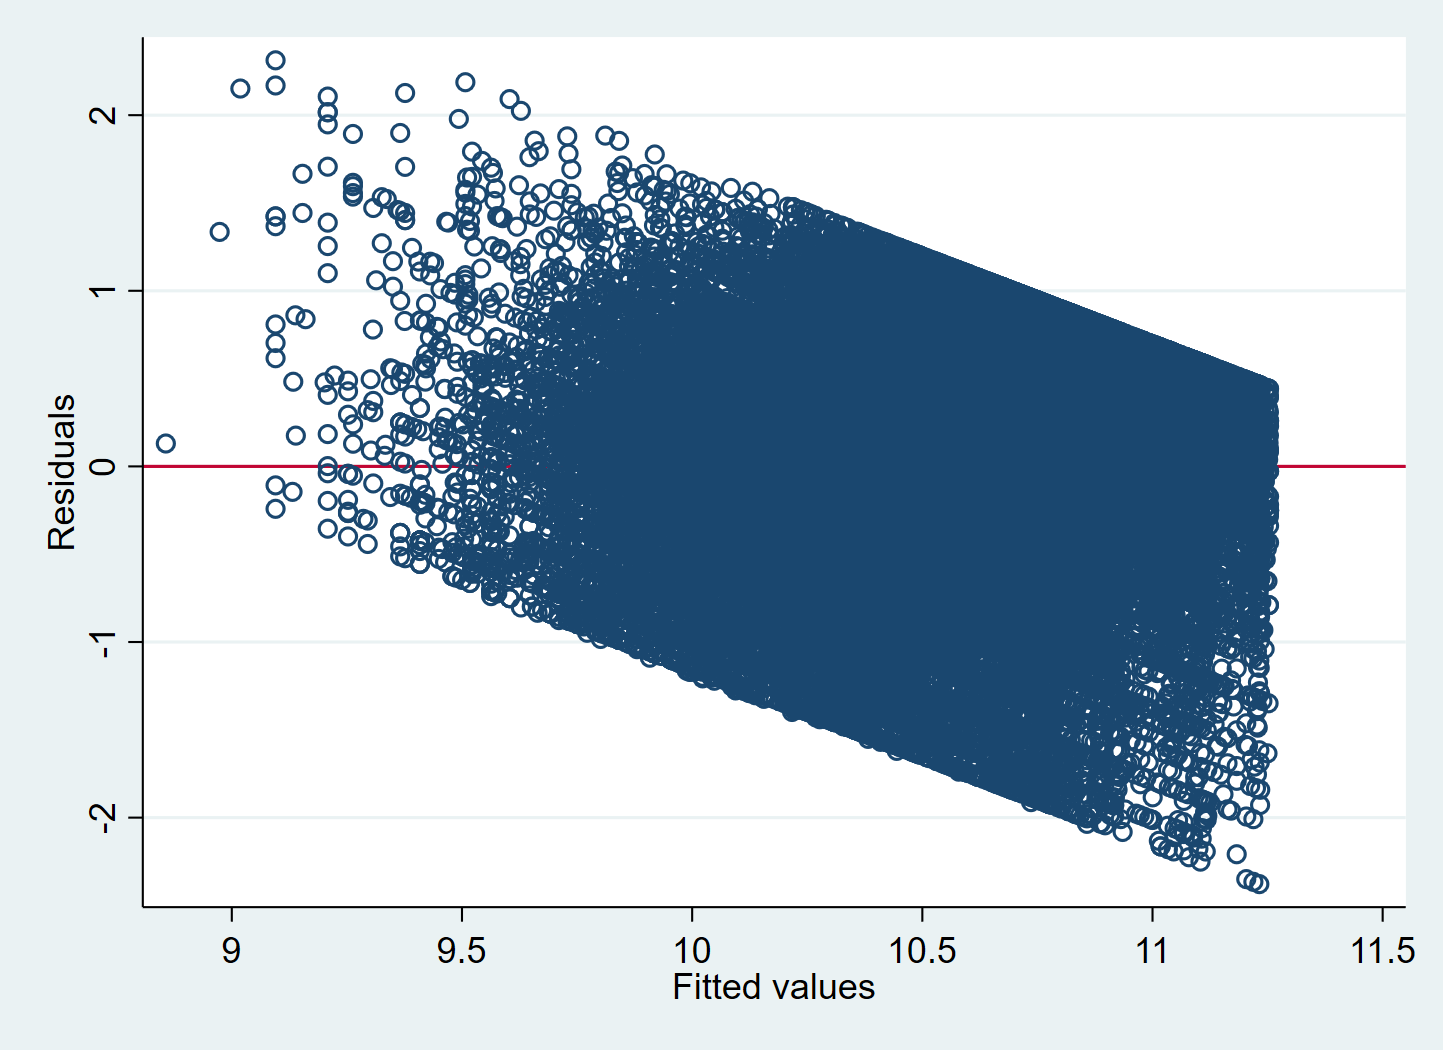
\includegraphics[scale=0.2]{{figures/graph_rvfplot}}
  \caption{\label{fig:rvfplot}
  \textit{rvfplot}\protect\footnotemark of fitted values and residuals
   }
\end{figure}

\footnotetext{\textit{rvfplot} is a Stata command used to graph a residual-versus-fitted plot, a graph of the residuals against the fitted values.}



\subsubsection{Large outliers are unlikely}\label{appendix:outliers}
Mathematically speaking, we say that it is unlikely to have large outliers if
\[
0<\mathop{\mathbb{E}}[\,X_{1i}^4\,]<\infty \quad \eqcomma \dotsm \eqcomma \quad 0<\mathop{\mathbb{E}}[\,X_{ki}^4\,]<\infty\eqcomma \quad and \quad 0<\mathop{\mathbb{E}}[\,Y_{i}^4\,]<\infty
\]
We already cleaned our data set by using Box-and-Whisker plots as mentioned in \hyperref[sec:data]{\text{Data}} section. Another way to state this assumption is that $X$ and $Y$ have finite kurtosis \cite{stock_watson_2019}. We found that all variables have a finite kurtosis using Stata, though we reject the hypothesis that the kurtosis is normal (See Table \ref{tab:im}).

\subsubsection{Normal errors}\label{appendix:normality}
Normal errors refer to the normality of our error term $\epsilon$:
\[
\epsilon \sim \mathcal{N}(0,\,\sigma^{2})
\]
In multivariate regression, \acs{CLT} applies to the \acs{OLS} estimators as well \cite{christopher_2006, stock_watson_2019}. \ie\,$\hat{\beta_{i}} \sim \mathcal{N}(\beta_{i},\,\sigma^{2}_{\hat{\beta_{i}}})$. In our case, since the model is heteroscedastic, it is hard to conclude that the errors are normal \cite{wooldridge_2020}. However, we can observe the error follows asymptotic normality in some extent in Figure (\ref{fig:rvfplot}). When sample size is large, the distributions of the regression coefficients approach normality under general conditions \cite{kuter_nachtsheim_neter_li_2005}.

\section{Acronyms}
\begin{multicols}{2}
\begin{acronym}[OWL-QN]

\acro{BLUE}{Best Linear Unbiased Estimator}
\acro{CLM}{Classical Linear Model}
\acro{CLT}{Central Limit Theorem}
\acro{CPS}{Community Population Survey}
\acro{GMT}{Gauss-Markov Theorem}
\acro{i.i.d}{independent and identically distributed}
\acro{MLR}{Multiple Linear Regression Model}
\acro{MNR}{Multiple Nonlinear Regression Model}
\acro{MVUE}{Minimum-Variance Unbiased Estimator}
\acro{OLS}{Ordinary Least Squares}
\acro{OVB}{Omitted Variable Bias}
\acro{PRF}{Population Regression Function}
\acro{RESET}{Regression Specification Error Test}
\acro{SRF}{Sample Regression Function}

\end{acronym}
\end{multicols}

\end{appendices}

\bibliographystyle{plain}
\bibliography{bibliography}

\end{document}
